\chapter{Chapter 1}


\section{Section}

A TABLE\footcite{APPLE1:ONLINE}

\begin{table}[h]
\centering

\counterwithout{figure}{chapter} 
\counterwithout{table}{chapter} 

\begin{tabularx}{\textwidth}{|lX|}
\hline
\rowcolor{gray!50} \textbf{Methoden Name} & \textbf{Funktion} \\ 
GET  & Ruft die Information ab, die unter der angebenen Request-\ac{URI} spezifiziert ist \\ 
POST  & Schickt eine unbegrenzte Menge an Daten zur Verarbeitung an den Server (abhängig von der Servereinstellung) \\ \hline
HEAD & Ruft nur den Header für die Request-\ac{URI} ab und bietet so die Möglichkeit zu vergleichen, ob eine Ressource sich zwischenzeitlich verändert hat \\ 
PUT & Bietet die Möglichkeit eine lokale Datei unter Angabe einer \ac{URI} an den Webserver zu senden \\ 
\hline
\end{tabularx}
\caption{Die vier gebräuchtlichsten Request Methoden}
\label{tab:http2}
\end{table}

\counterwithout{lstlisting}{chapter} 

\lstset{language=PHP}
\lstinputlisting[caption={Sourcecode 1}]{sourcecode/test.php}

\counterwithout{figure}{chapter} 
\begin{figure}[h]
\centering
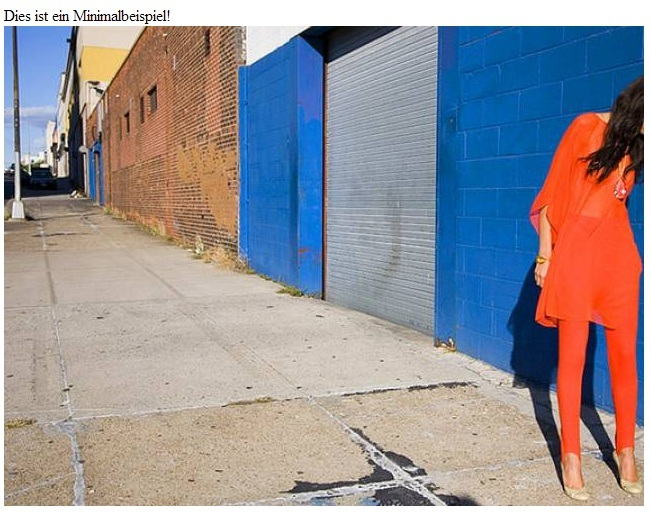
\includegraphics[width=\textwidth]{images/abt1_webseite.jpg}
\caption{Figure 1}
\end{figure}


